\documentclass{standalone}
\usepackage{tikz}
\usetikzlibrary{shapes.geometric, arrows}

\tikzstyle{startstop} = [rectangle, rounded corners, minimum width=3cm, minimum height=1cm,text centered, draw=black, fill=red!30]
\tikzstyle{io} = [trapezium, trapezium left angle=70, trapezium right angle=110, minimum width=3cm, minimum height=1cm, text centered, draw=black, fill=blue!30]
\tikzstyle{process} = [rectangle, minimum width=3cm, minimum height=1cm, text centered, draw=black, fill=orange!30]
\tikzstyle{decision} = [diamond, minimum width=3cm, minimum height=1cm, text centered, draw=black, fill=green!30]

\tikzstyle{arrow} = [thick,->,>=stealth]


\begin{document}


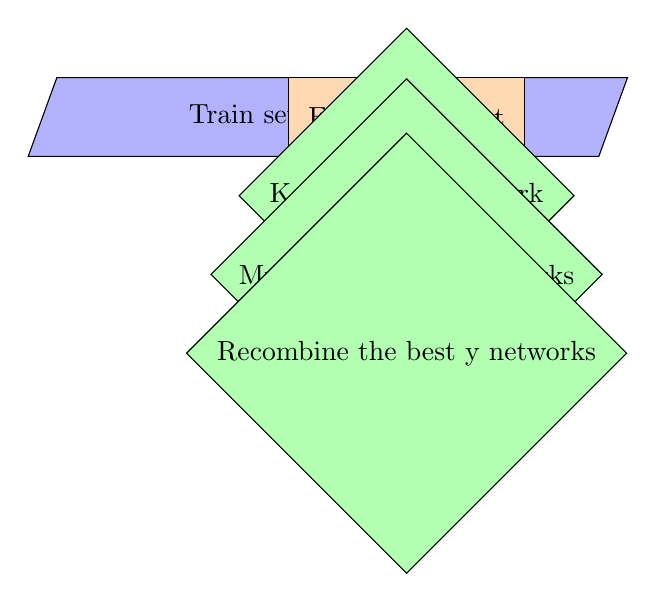
\begin{tikzpicture}
    \node (start) [startstop] {Set of random neural networks};
    \node (train) [io, right of=start] {Train set for 25 epochs};
    \node (eval)  [process, right of=train] {Evaluate the set};
    \node (keep)  [decision, below of=eval] {Keep the best network};
    \node (mutate)  [decision, below of=keep] {Mutate the best x networks};
    \node (recombine)  [decision, below of=mutate] {Recombine the best y networks};
\end{tikzpicture}
    
\end{document}